\chapter{System architecture and Methods}\label{ch:architecture}


%2nd-review
In this chapter, we will present developed tool, called SIMITAR: SnIffing, ModellIng and TrAffic geneRation, and how it works. First, we will discuss its architecture and components. Then we will present a brief tutorial of how to expand its support for a traffic generator engine. 

%2nd-review
We abstract its whole operation cycle in the figure ~\ref{fig:cycle-of-operation}. Our tool, from live captures or \textit{pcap} file collects raw data from Ethernet traffic. It then breaks these data into different flows. It uses this data to generate a set of parameters for our traffic models, using a set of algorithms. Finally, it provides these parameters to a traffic generator engine and controls its packets injection.

% cycle of operation
%2nd-review
\begin{figure*}[ht!]
        \centering
        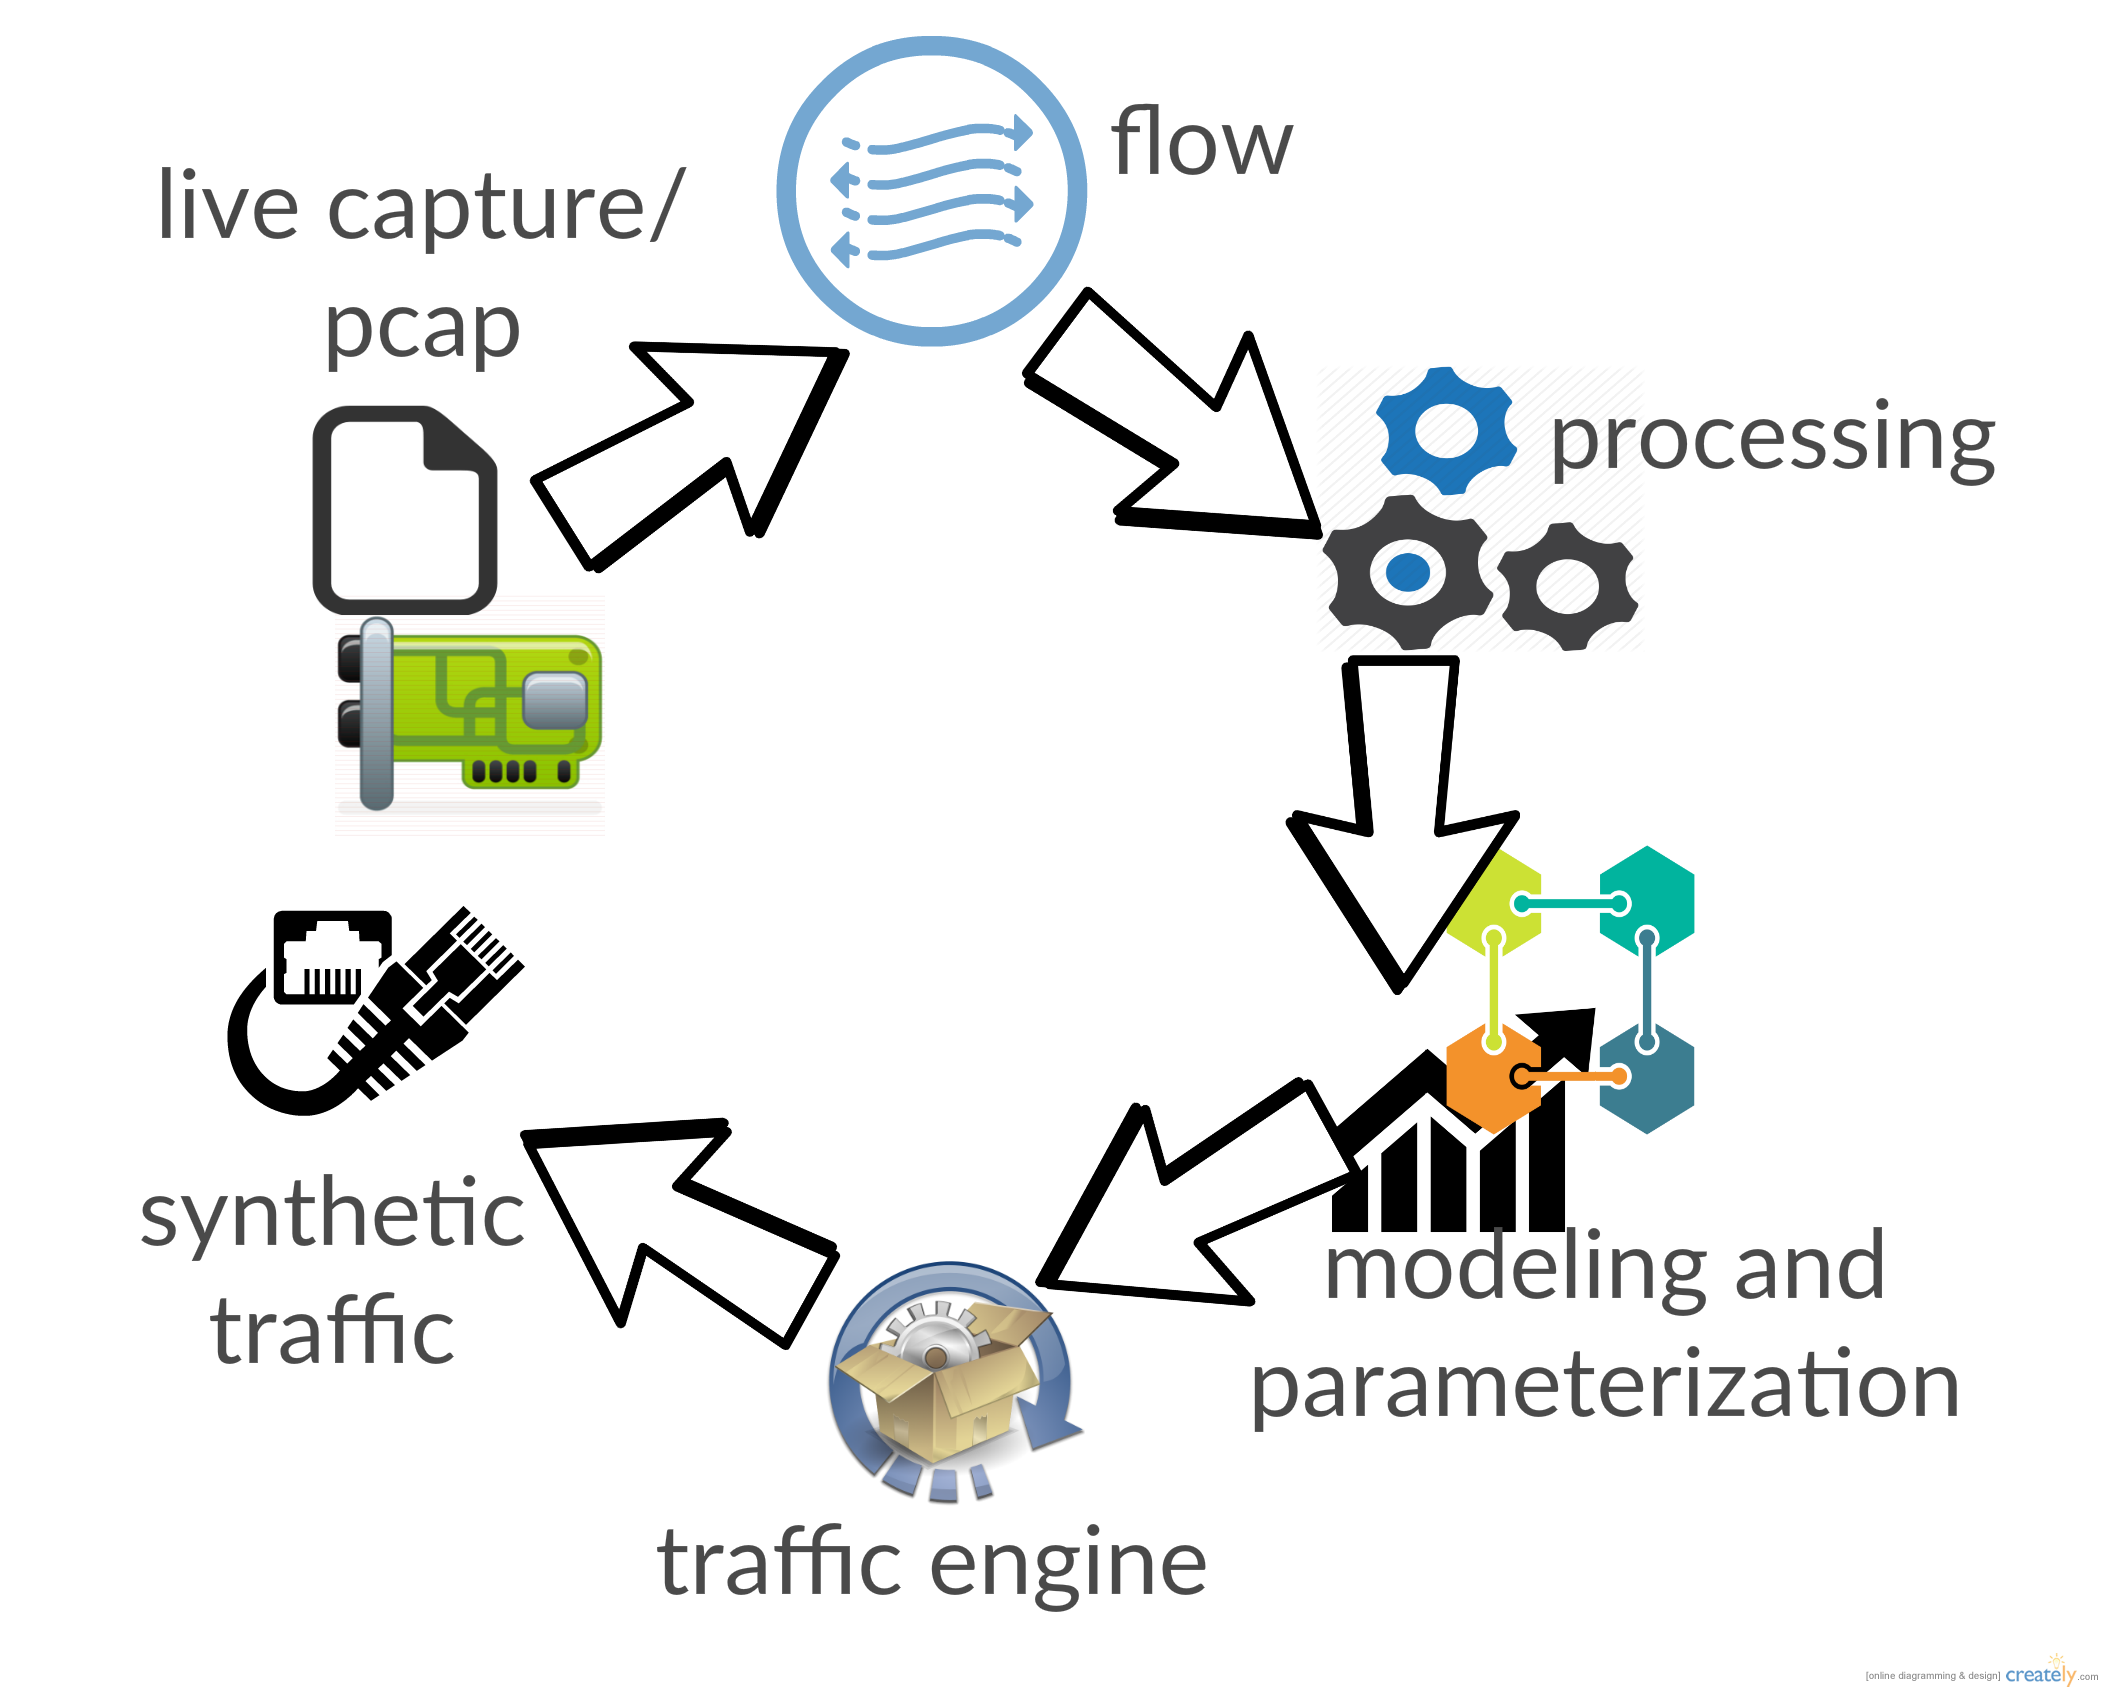
\includegraphics[height=3.0in]{figures/ch3/digram-project-cycle}
        \caption{This figure represents an operation cycle of SIMITAR, emphasizing each main step: sniffing, flow classification, data storing, data processing and fitting, model parameterization,  and synthetic traffic generation.}
    \label{fig:cycle-of-operation}
\end{figure*}


\section{SIMITAR Architecture}

%2nd-review
To meet the requirements presented in the section ~\ref{ch:introduction}, we will present a solution, and define how each part works, as in a low-level requirement list\cite{sommerville}.  

%2nd-review
SIMITAR architecture is presented in the figure~\ref{fig:architecture}, and it is composed of five components: a \textit{Sniffer}, a \textit{SQLite database}, a \textit{TraceAnalyzer}, a \textit{FlowGenerator} and the \textit{Network Traffic Generator}, as subsystem. We describe each part below.

% component diagram and module design
\begin{figure*}[ht!]
        \centering
        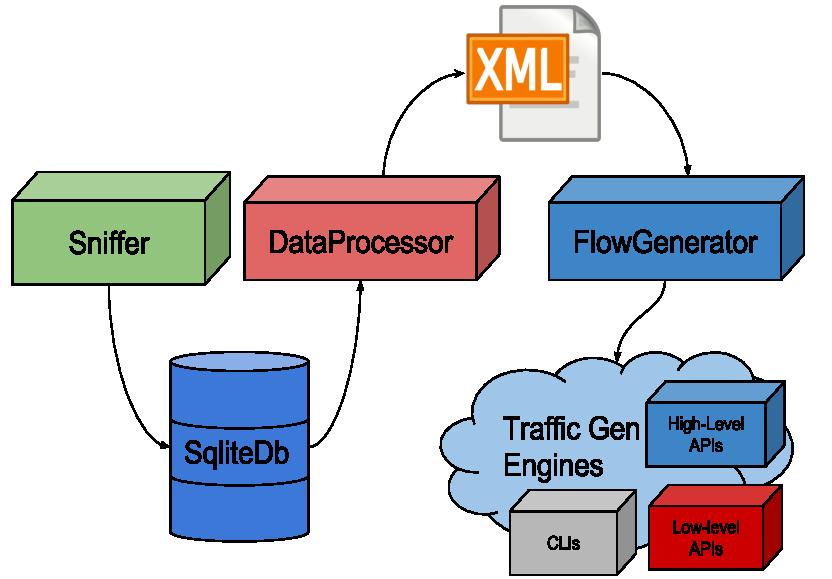
\includegraphics[height=2.7in]{figures/ch3/architecture-diagram}
        \caption{Architecture of SIMITAR}
    \label{fig:architecture}
\end{figure*}



%%%%%%%%%%%%%%%%%%%%%%%%%%%%%%%%%%%%%%%%%%%%%%%%%%%%%%%%%%%%%%%%%%%%%%%%%%%%%%%%
\subsection{Sniffer}

%2nd-review
This component collects network traffic data and classifies it into flows, storing stores in an SQLite database. It defines each flow by the same criteria used by SDN switches\cite{sdn-survey}, through header fields matches (Link Protocol, Network Protocol, Network Source Address, Network Destination Address, Transport Protocol, Transport Source Port, Transport Destination Port). It can work over a \textit{pcap} file or over an Ethernet interface. 

\begin{figure*}[ht!]
        \centering
        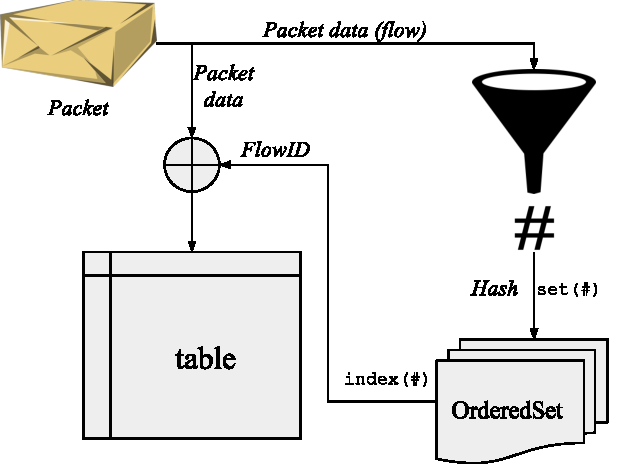
\includegraphics[height=2.5in]{figures/ch3/sniffer-classifier}
        \caption{SIMITAR's sniffer hash-based flow classification}
    \label{fig:sniffer}
\end{figure*}

%2nd-review
The first version of this component was implemented in Shell Script (Bash).  Tsahrk\footnote{\href{https://www.wireshark.org/docs/man-pages/tshark.html}{https://www.wireshark.org/docs/man-pages/tshark.html}} was used to extract header fields, and Awk to match the flows, and Sed/Awk to create the Sqlite queries. This version was too slow to operate in real time on Ethernet interfaces. On the other hand, was fast to implement, and enable the implementation of the other components, before this final version was released.

%2nd-review
The second version was implemented using Python. This version used Pyshark\footnote{\href{https://pypi.python.org/pypi/pyshark}{https://pypi.python.org/pypi/pyshark}} as sniffer library. The flow classification is made by a class called FlowId. It contains class we developed called OrderedSet. A set is a list of elements with no repetition, but do not keep track of the insertion order. But our OrderedSet does. Also, it make use of a  32 bits hash function of the family FNV. The listed header fields are inputs for a hash function, its value is set on the ordered set, and its order is returned. This value is set as a packet flowID.  

%c++ http://ideone.com/F0V42m
%2nd-review
As future improvements for this component, we propose a more efficient implementation in C++ and data visualization for the collected data. We discuss this in deeper details in the chapter~\ref{ch:conclusion}




%%%%%%%%%%%%%%%%%%%%%%%%%%%%%%%%%%%%%%%%%%%%%%%%%%%%%%%%%%%%%%%%%%%%%%%%%%%%%%%%
\subsection{SQLite database}

\begin{figure*}[ht!]
        \centering
        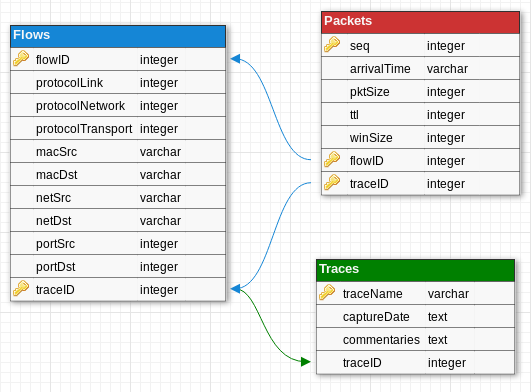
\includegraphics[height=2.5in]{figures/ch3/database-relational-model}
        \caption{SIMITAR's SQLite database relational model}
    \label{fig:simitar-database}
\end{figure*}

%2nd-review
The database will store the collected raw data for further analysis. It is responsible for storing data from different traces in different tables.  The \textit{Sniffer} and the \textit{TraceAnalyzer}  can access the database. 

%2nd-review
We choose an SQLite database, because according to the SQLite specifications\footnote{\href{https://www.sqlite.org/whentouse.html}{https://www.sqlite.org/whentouse.html}}, it is the best option for our database. It is simple and well-suitable for an amount of data smaller than terabytes.

%2nd-review
In the figure ~\ref{fig:simitar-database} we present the relational model of our database, which stores a set of features extracted from the packets, along with the FlowID calculated by the sniffer component. 


\subsection{Trace Analyzer}

%2nd-review
This module is the core of our project. It creates a compact trace descriptor via the analysis of the collected data. We define here a Compact Trace Descriptor (CTD) as a human and machine readable file, which describes an original traffic trace trough a set of flows, each of them described by a set of parameters, like header information and analytical models. 

%2nd-review
Therefore, the Trace Analyze learns the features from raw data of traces (stored in the SQLite database) and write them in an XML file.  In the figure~\ref{fig:CTD-diagram} we show a directory diagram of a CDT file. It has many of many flow fields, and each one contains each parameter estimated. 

%\begin{figure*}[!ht]
%    \centering
%    \begin{subfigure}[t]{0.45\textwidth}
%        \centering
%        \includegraphics[height=2.5in]{figures/03_compact_trace_descriptor_tree_structure}
%        \caption{caption}
%    \end{subfigure}%
%    ~ 
%    \begin{subfigure}[t]{0.45\textwidth}
%        \centering
%        \includegraphics[height=2.5in]{figures/03_compact_trace_descriptor_tree_structure_2}
%        \caption{caption}
%    \end{subfigure}
%    \caption{caption}
%    \label{fig:CTD-diagram}
%\end{figure*}
%height=2.5in
%

%2nd-review
\begin{figure}
\centering
\subfloat[first]{
  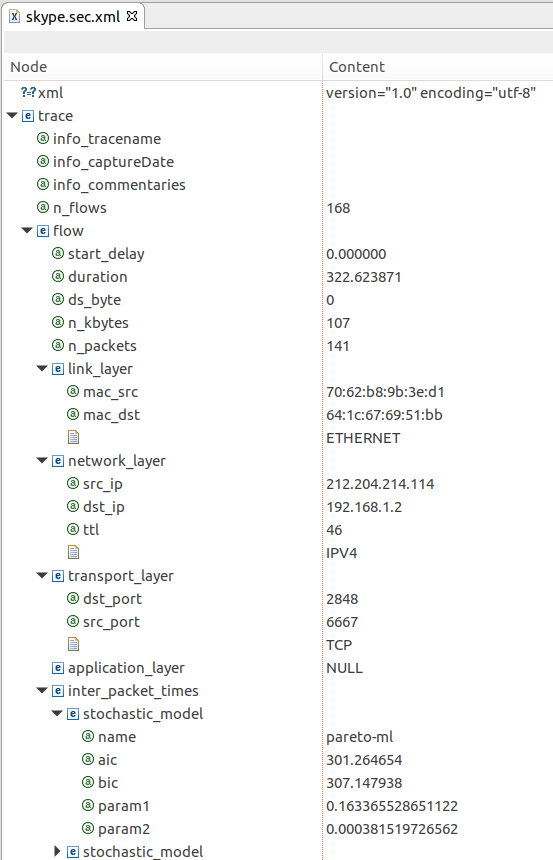
\includegraphics[height=4.in]{figures/ch3/cdt1}
}
\subfloat[second]{
  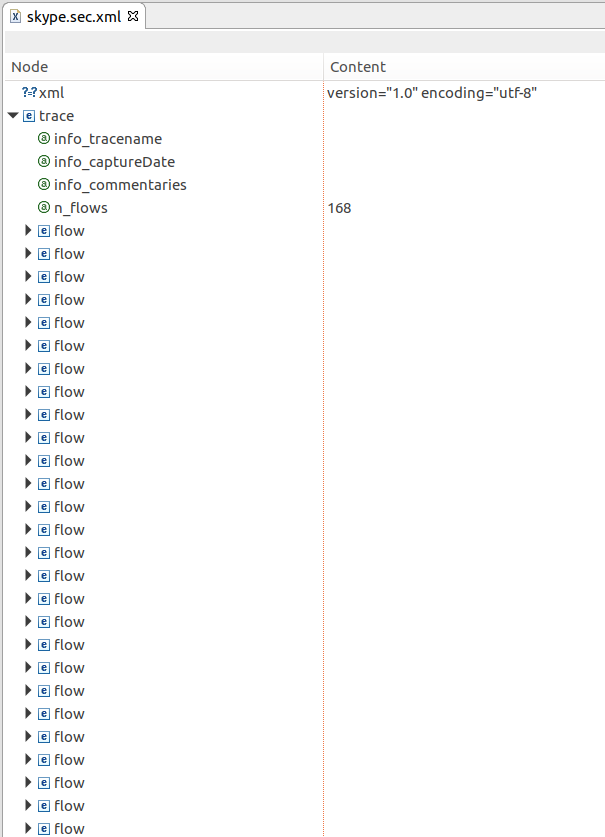
\includegraphics[height=4.in]{figures/ch3/cdt2}
}
\caption{Directory diagram of the schema of a Compact Trace Descriptor (CDT) file. On the left, we present a dissected flow, and on the right a set of flows.}
\label{fig:CTD-diagram}
\end{figure}


\subsubsection{Flow features}

%2nd-review
Some features are unique per flow and can be directly measured from the data. They are:  

%2nd-review
\begin{itemize}
\item Flow-level properties like duration of flow, start delay, number of packets per flow, number of KBytes per flow;
\item Packet-level QoS metrics like bit rate and packet rate; 
\item Header fields, like protocols (IPv4, IPv6, TCP, UDP, ICMP, DCCP, SCTP, etc), QoS fields, ports, and addresses.
\end{itemize}

%2nd-review
Each one of these parameters is unique per flow. Other features like PSD (packet size distribution) e IPT (Inter-packet time), have a more complex behavior.  To represent these characteristics, we will use sets of stochastic-based models.  

\subsubsection{Inter Packet Times}

\begin{figure*}[ht!]
    \centering
    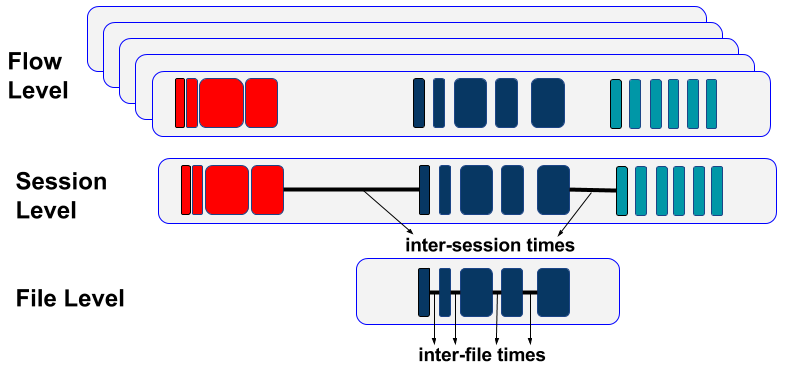
\includegraphics[height=2.0in]{figures/ch3/modified-harpoon-model}
    \caption{The schema of the modified version of the Harpoon algorithm we adopt on SCIMITAR.}
    \label{fig:modified-harpoon-model}
\end{figure*}

%2nd-review
To represent IPT, we adopt a simplified version of the Harpoon traffic model. A deep explanation of the original model can be found at \cite{harpoon-paper} and \cite{harpoon-validation}. Here, we will explain our simplified version, which is illustrated at figure~\ref{fig:modified-harpoon-model}. 

%2nd-review
Harpoon uses a more conventional definition of each level, based on the measurement of SYN and ACK TCP flags. Harpoons use TCP flags (SYN) to classify packets in different levels (named there: file, session and user level). Since we are just modeling inter-packet times, we choose to estimate these values, based on inter-packet times. Since we want to generalize this approach for any protocol, the distinction will be made based on the time delay between packets.

%2nd-review
In our version of the algorithm, we define (as Harpoon does) three different layers of data transference to model and control: file, session, and flow. 

%2nd-review
For SIMITAR, a file is just a sequence of consecutive packets transmitted continuously, without large interruption of traffic. It can be, for example, packets transmitted downloading a file, of UDP packets of a connection or a single ICMP echo packet. The session-layer refers to a sequence of multiple files transmitted between a source and a destination, belonging to the same flow.  And the flow level refers to the conjunct of flow classified by the Sniffer.  

%2nd-review
\textbf{Flow-layer}: The Trace Analyzer loads the flow arrival times from the database, and calculates the inter-packet times within the flow context. 

%2nd-review
\textbf{Session-layer}: At the session layer, we use a deterministic approach for evaluating times between transferred files (OFF times) and the actual file transference (ON times). It is basically a deterministic ON/OFF model. We choose a deterministic model because in this way we can express diurnal behavior\cite{harpoon-paper}.  We develop an algorithm called \textit{calcOnOff} responsible for estimating these times. It also determines the number of packets and bytes transferred by each file. Since the on times will serve as input for actual traffic generators, we defined a minimum acceptable time for on periods equals to 100 ms. We did this, first because ON times can be arbitrary smalls, and they could be incompatible with acceptable ON periods for traffic generators. Second, because in the case of just one packet, the ON time would be zero. OFF times, on the other hand, are defined by the constant \texttt{m\_session\_cut\_time}. If the time between packets of the same flow is larger than this, we consider it belonging to a different file, so it is a Session OFF time. In this case, we use the same value of the constant \textit{Request and Response timeout} of Swing\cite{swing-paper} (30 seconds) \textcolor{red}{<<<<pode mudar, calibrar>>>>}.
The control of ON/OFF periods is made by the \texttt{NetworkFlow} class.

%2nd-review
\textbf{File-layer}: Here we model the inter-packet times at the file level. To estimate inter-packet times within files, we select all inter-packet times smaller than \texttt{m\_session\_cut\_time}. All files within the same flow are considered to follow the same model. We delegate the control of the inter-packet times to the underlying workload engine tool. We ordered them, from the best to the worst. Currently, we are using eight different stochastic functions parameterizations. They are Weibull(linear regression), Normal(mean/standard deviation calculation), Exponential(mean and linear regression estimation), Pareto(linear regression and maximum likelihood), Cauchy(linear regression) and Constant(mean calculation). From those, Weibull, Pareto, and Cauchy are heavy-tailed functions, and therefore self-similar processes. \textcolor{red}{<<<<pode mudar, calibrar>>>>} But if the flow has less than 30 packets, just the constant model is evaluated. It is because numerical methods gave poor results if the data sample used is small. We sort these models according to the Akaike Information Criterion (AIC)\cite{sourcesonoff-paper}\cite{bic-aic-comparision}. We will enter in deeper details on this methodology on the chapter ~\ref{ch:modeling-evaluation}. The methodology of selection is presented in the figure~\ref{fig:model-parameterization}

%2nd-review
\begin{figure*}[ht!]
    \centering
    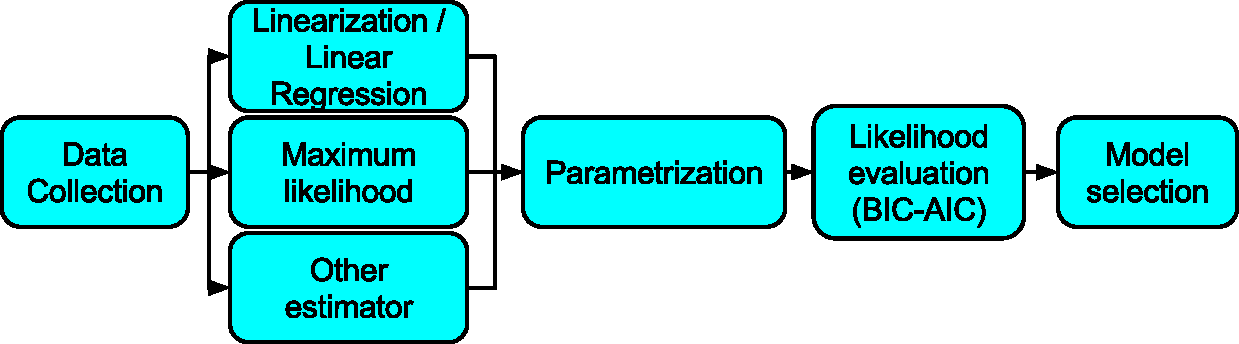
\includegraphics[height=1.6in]{figures/ch3/ipt-modeling}
    \caption{Diagram of parameterization and model selection for inter-packet times and inter-file times.}
    \label{fig:model-parameterization}
\end{figure*}

%\begin{figure*}[ht!]
%    \centering
%    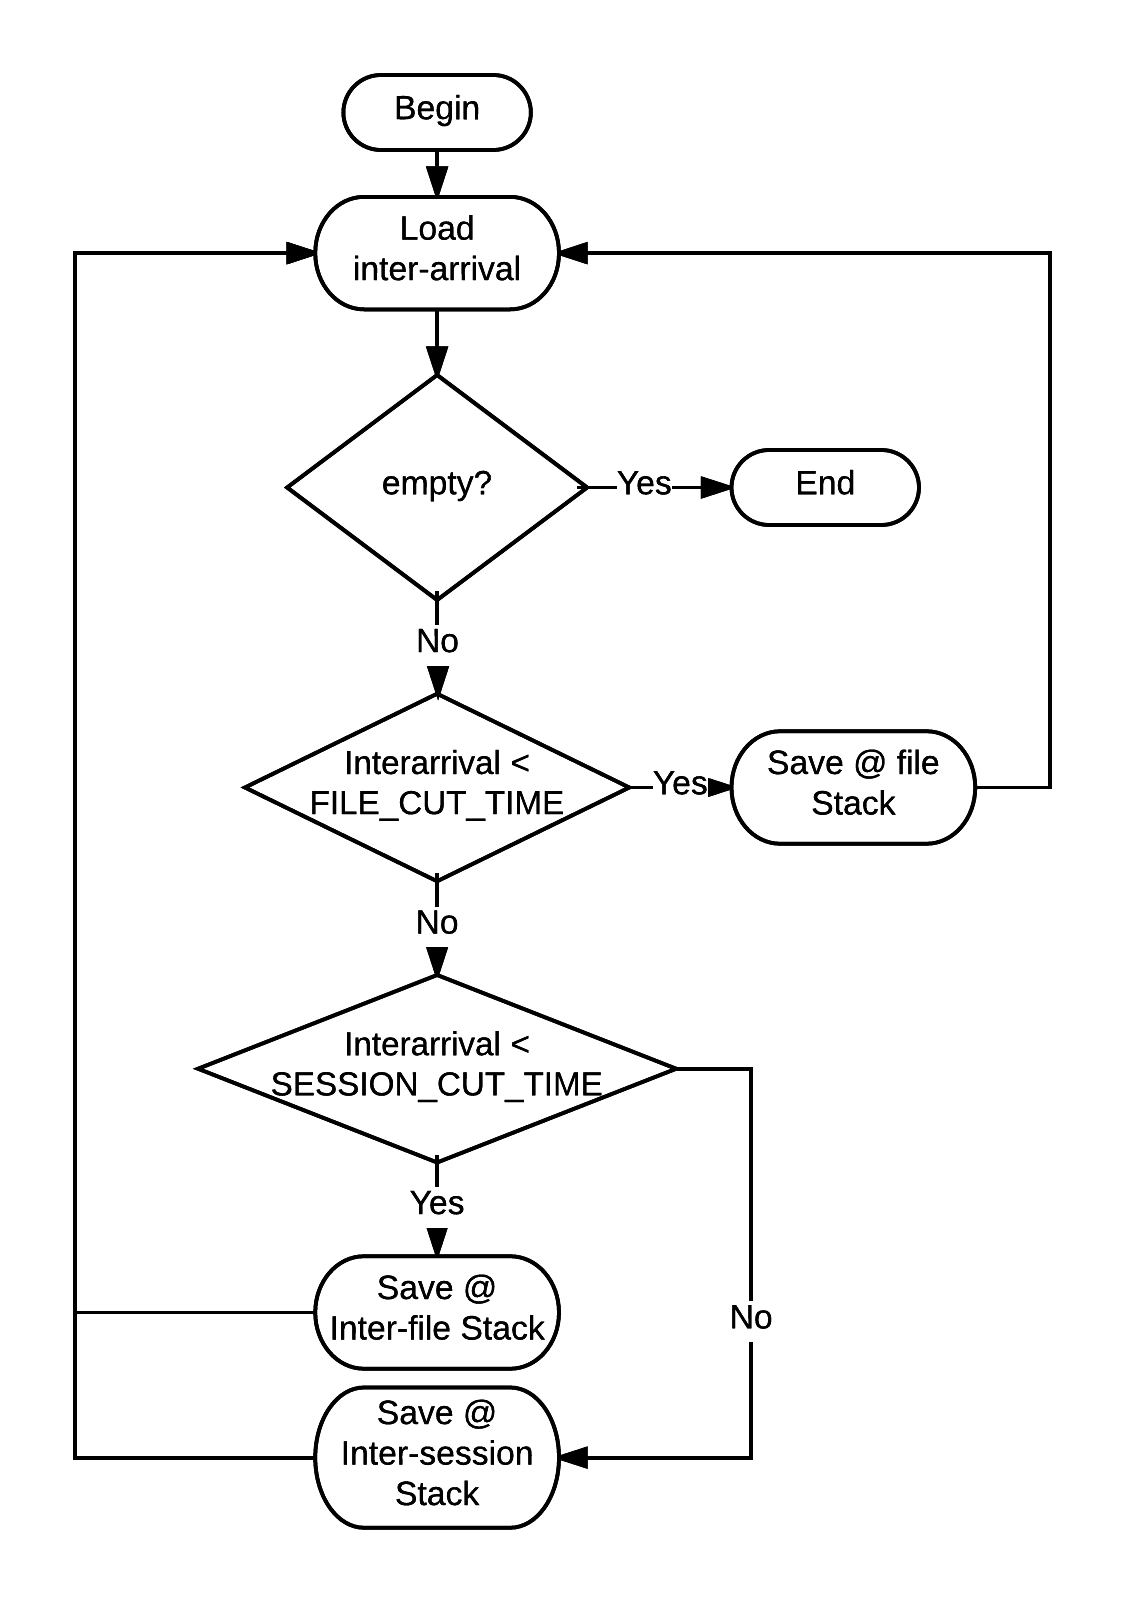
\includegraphics[height=4.0in]{figures/ch3/alg-paremeterization}
%    \caption{caption.}
%    \label{fig:harpoon-alg-times-estimator}
%\end{figure*}

\subsubsection{Packet Sizes}

%2nd-review
Our approach for the packet size is much simpler. Since the majority of packet size distribution found on real measurements are bi-modal \cite{packet-distribution-model}\cite{sourcesonoff-paper}\cite{udp-flows-model}, we first sort all packet sizes of flow in two modes. We define a packet size mode cut value of 750 bytes, same value adopted by \cite{udp-flows-model}. 

%2nd-review
We first know how much packets each mode has, and then we fit a model for it. We use three stochastic models: constant, exponential and normal. Since self-similarity is not a requirement, we prefer to use just simple models. But, when there is no packet we set a flag NO\_MODEL, and when there is just a single packet we just use the constant model.  We then calculate the BIC and AIC for each of them and sort according to the AIC value by default, but we decide to set the constant model as the first.

%2nd-review
As is possible to see on many studies \cite{packet-distribution-model}\cite{udp-flows-model}, since the standard deviation of each mode is small, constant fittings use to give good approximations. Also, it is computationally cheaper than the others models, since no calculation is a need for each packet sent. Since both AIC and BIC criteria always will select the constant model as the worst, we decide to ignore this indicator for the constant model.

\subsubsection{Compact Trace Descriptor}

%2nd-review
An example of the final result of all the methods is presented in the XML code down below. It illustrates a flow of a \textit{Compact Trace Descriptor}(CDT) file.

\begin{minted}[frame=single,
               framesep=3mm,
               linenos=true,
               xleftmargin=21pt,
               tabsize=4,
               fontsize=\scriptsize, 
               breaklines=true]{xml}
<flow start_delay="31.621941" duration="91.584654" ds_byte="0" n_kbytes="1" n_packets="13">
	<link_layer mac_src="no-mac-src" mac_dst="no-mac-dst">ETHERNET</link_layer>
	<network_layer src_ip="10.1.1.48" dst_ip="216.58.199.35" ttl="64">IPV4</network_layer>
	<transport_layer dst_port="34683" src_port="443">TCP</transport_layer>
	<application_layer>HTTPS</application_layer>
	<inter_packet_times>
		<stochastic_model name="pareto-ml" aic="-24.738412" bic="-23.768599" param1="0.152500524612205" param2="0.000024050000003"/>
		<stochastic_model name="weibull" aic="-16.155977" bic="-15.186164" param1="0.130469107098031" param2="0.063433369086366"/>
		<stochastic_model name="pareto-lr" aic="49.322192" bic="50.292005" param1="0.892551148108768" param2="0.000024050000003"/>
		<stochastic_model name="exponential-me" aic="76.776570" bic="77.746383" param1="0.131026317153354" param2="0.000000000000000"/>
        <stochastic_model name="normal" aic="105.882623" bic="106.852436" param1="7.632054549999999" param2="17.598918053235813"/>
        <stochastic_model name="exponential-lr" aic="116.913056" bic="117.882870" param1="0.009752000000000" param2="0.000000000000000"/>
        <stochastic_model name="cauchy" aic="128.406532" bic="129.376345" param1="1.935832000000000" param2="-7.245692000000000"/>
        <stochastic_model name="constant" aic="inf" bic="inf" param1="7.632054549999999" param2="0.000000000000000"/>
    </inter_packet_times>
	<session_times on_times="0.96856400,0.10000000,0.10000000" off_times="45.30807900,45.30801100" n_packets="11,1,1" n_bytes="1650,66,66"/>
	<packet_sizes n_packets="13" n_kbytes="1">
		<ps_mode1 n_packets="12" n_kbytes="1">
			<stochastic_model name="constant" aic="inf" bic="inf" param1="99.916667" param2="0.000000"/>
			<stochastic_model name="normal" aic="137.020397" bic="137.990210" param1="99.916667" param2="64.408439"/>
			<stochastic_model name="exponential-me" aic="138.504076" bic="139.473889" param1="0.010008" param2="0.000000"/>
		</ps_mode1>
		<ps_mode2 n_packets="1" n_kbytes="0">
		<stochastic_model name="constant" aic="inf" bic="inf" param1="583.000000" param2="0.000000"/>
		</ps_mode2>
	</packet_sizes>
</flow>
\end{minted}

%2nd-review
The current version of our tool, do not intrinsically supports responsiveness. The underlying traffic generator API can support it (such as Seagull\cite{web-seagull}), but we do not generate any mathematical model for this purpose, and this may also stand as a future work we discuss on chapter ~\ref{ch:conclusion}. 

\subsection{Flow Generator}

\begin{figure*}[ht!]
    \centering
    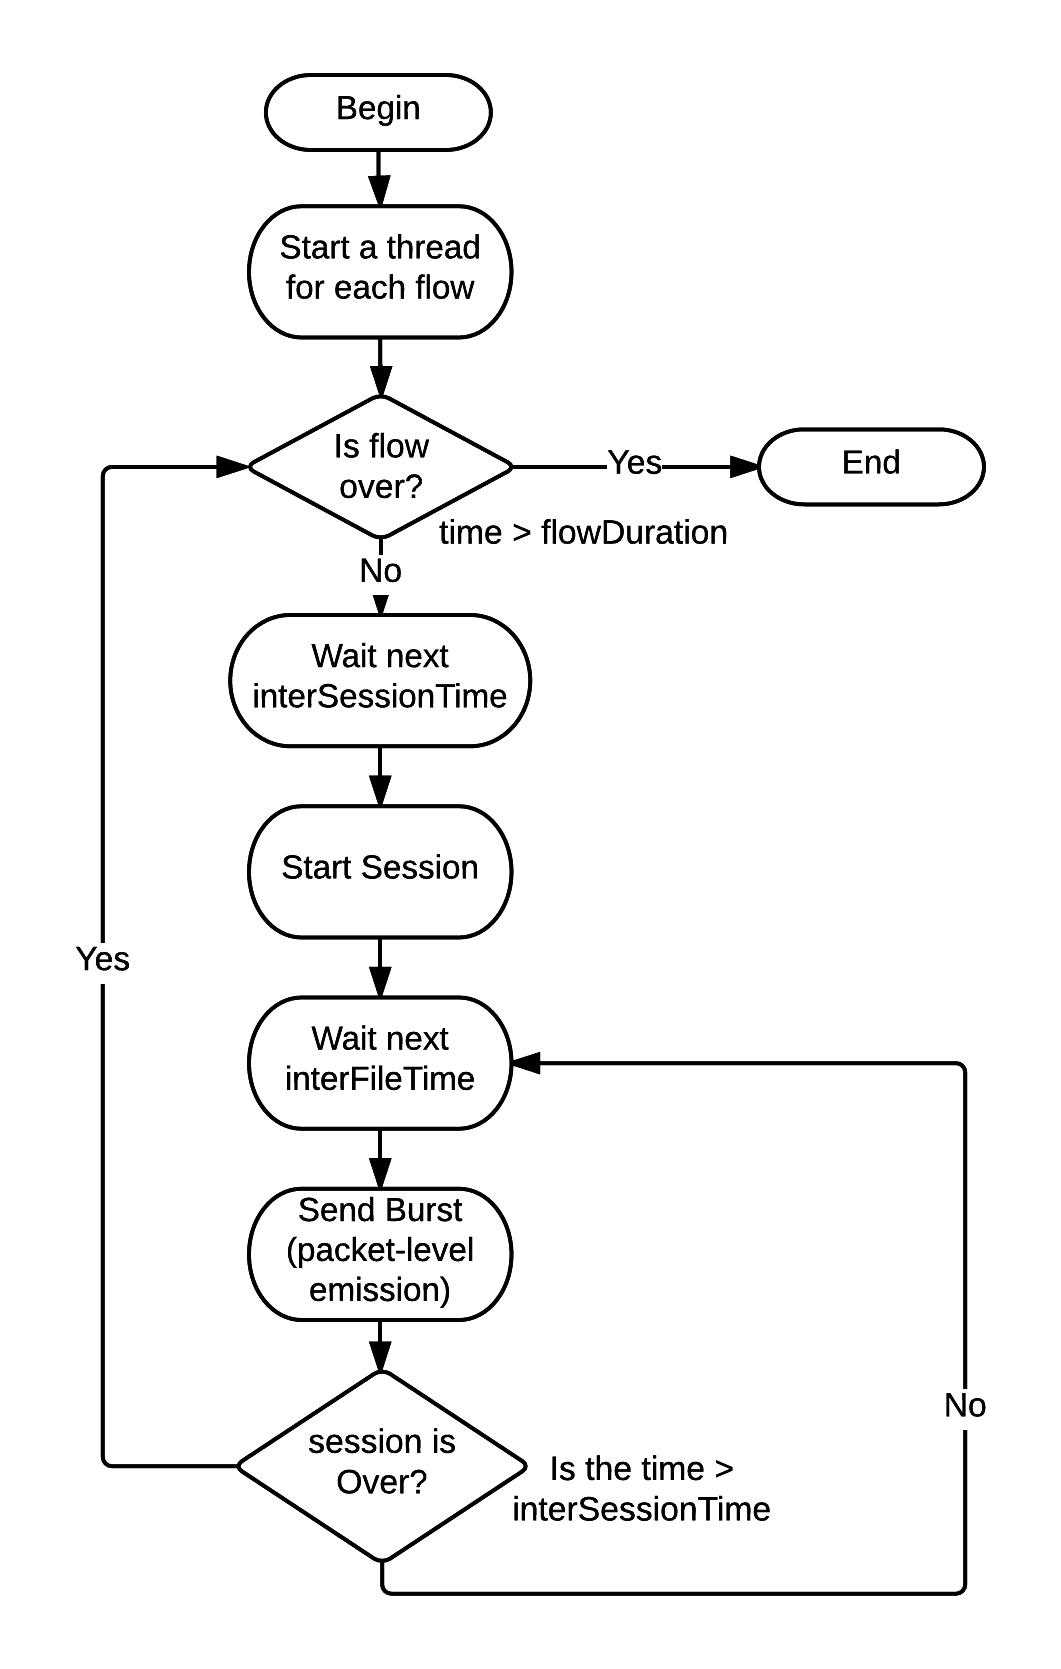
\includegraphics[height=4.0in]{figures/ch3/alg-simplified-harpoon}
    \caption{Simplified-harpoon emission algorithm}
    \label{fig:alg-simplified-harpoon}
\end{figure*}

%2nd-review
The Flow Generator handles the data on the CTD file, and use it as parameters for the traffic generation. It crafts and controls each flow in a separated thread. 

%2nd-review
We first implemented it using the D-ITG API. But our Flow Generator can use any traffic generator with API, CLI or script interface as well. To easily expand this component, we use the design pattern factory. If the user wants to introduce support for a new traffic generator, he just has to expand the class \texttt{DummyFlow} and add the support on the method \texttt{make\_flow()} of the class \texttt{NetworkFlow}. We will discuss this deeper in the next section.

%2nd-review
This component works in two different layers according to the traffic generators classification introduced in the chapter ~\ref{ch:literature-review}: at the Flow level, and packet level, as presented in the figure ~\ref{fig:layers-workload-tools}. 

\begin{figure*}[ht!]
    \centering
    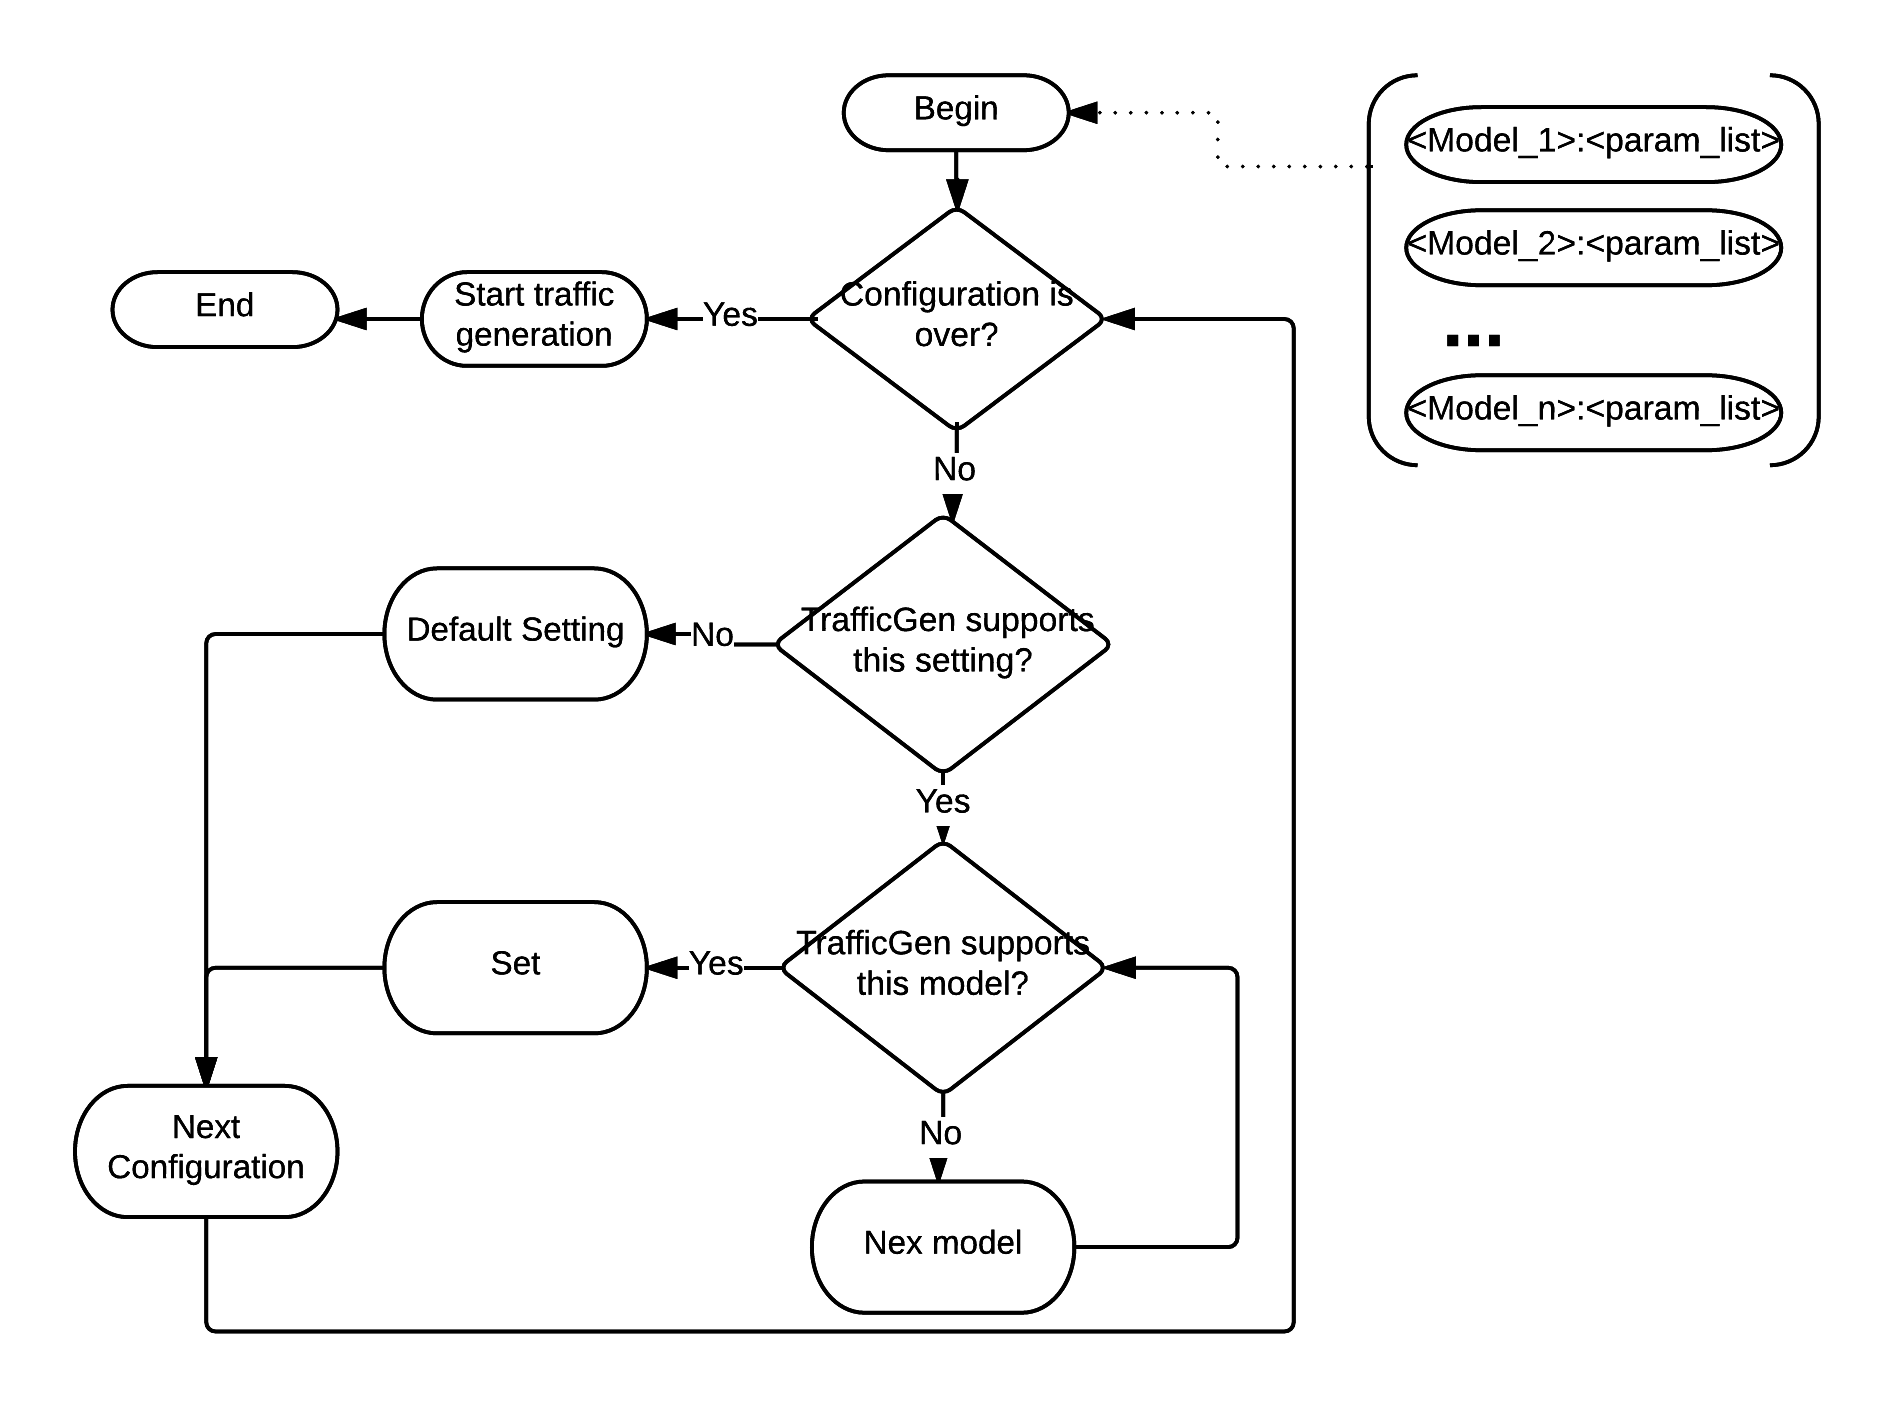
\includegraphics[height=4.0in]{figures/ch3/alg-traffic-engine-config}
    \caption{Traffic engine configuration model}
    \label{fig:alg-traffic-engine-config}
\end{figure*}

\subsubsection{Flow-level Traffic Generation Operation}

%2nd-review
At the flow level, it controls each flow using the algorithm at figure~\ref{alg-simplified-harpoon}. This algorithm basically handles the our model defined at the figure~\ref{fig:modified-harpoon-model}.

%2nd-review
It starts a \textit{thread} for each flow in the \textit{Compact Trace Descriptor}, then the thread sleeps its \texttt{start\_delay}. It is the time when the first flow packet was captured in the original capture. it then calls the underlying traffic generation method, passing to it the file ON time, number of packets and number of bytes to be sent (file size). Then it sleeps the next Session-OFF time from the stack until it ends. When the list of ON/OFF times is over, the thread ends. The thread scheduling/joining is implemented by the class \texttt{NetworkTrace} and its sleep/wake process by the class \texttt{DummyFlow}.


\subsubsection{Flow Generation Programming}

%2nd-review
At the packet level, it must use the expanded class of the \texttt{DummyFlow}. In this level, the job of our tool is to configure the underlying engine, to send a file. Therefore it uses the \textit{getters} available, and the passed parameters, defined by the operation described in the previous session. The implementation of this level should follow the flowchart presented in the figure ~\ref{fig:alg-traffic-engine-config}.
Down below we present a simplistic code of how the D-ITG API can be used to generate packet-level traffic. We call this concept \textit{Flow Generation Programming} A more complex configuration is possible, but it serves to illustrate the procedure. Its API documentation is available at on D-ITG web-site \footnote{\href{http://www.grid.unina.it/software/ITG/manual/index.html\#SECTION00047000000000000000}{http://www.grid.unina.it/software/ITG/manual/index.html\#SECTION00047000000000000000}}. 
\begin{minted}[frame=single,
               framesep=3mm,
               linenos=true,
               xleftmargin=21pt,
               tabsize=4,
               fontsize=\scriptsize, 
               breaklines=true]{c++}
void flowGenerate(const counter& flowId, const time_sec& onTime, const uint& npackets, const uint& nbytes,  const string& netInterface)
{
	char localhost[CHAR_BUFFER];
	string strCommand;
	char command[CHAR_BUFFER];
	uint i = 0;
	int rc = 0;
	getLocalIp("eth0", localhost);
	strCommand += " -t " + std::to_string(onTime); 
	strCommand += " -k " + std::to_string(nbytes / 1024);
	strCommand += " -a " + getHostIP();
	if (this->getTransportProtocol() == PROTOCOL__TCP)
		strCommand += " -T TCP -D ";
	else if (this->getTransportProtocol() == PROTOCOL__UDP)
		strCommand += " -T UDP ";
	else if (this->getTransportProtocol() == PROTOCOL__ICMP)
		strCommand += " -T ICMP ";
	for(;;i++)
	{	
		StochasticModelFit idtModel = this->getInterDepertureTimeModel(i);
		if(idtModel.modelName() == WEIBULL)
		{
			strCommand += " -W " + std::to_string(idtModel.param1()) + " " + std::to_string(idtModel.param2());
			break;
		}
		else if ( idtModel.modelName() == CONSTANT)
		{
			strCommand += " -C " + std::to_string(nbytes/(1024*onTime));
			break;
		}
	}
	strcpy(command, strCommand.c_str());
	rc = DITGsend(localhost, command); // it is not blocking
    usleep(onTime*10e6);
	if (rc != 0)
	{
		printf("\nDITGsend() return value was %d\n", rc);
		exit(EXIT_FAILURE);
	}
}
\end{minted}

\subsection{Network Traffic Generator}


A network traffic generator software that should provide its API or script interface for the \textit{FlowGenerator} component. 
 
Since \texttt{DITGsend()} is thread safe, no mutex is need. It would be needed if a lower level API, such Libtins or Libpcap was used. In that case, these APIs would permit control precisely each packet sent through the interface, but a mutex would be necessary. An scriptable application, such as Iperf can be used as well, using \texttt{fork()} or \texttt{popen()}.

As we claimed before, this tools is simple of being expanded for almost any traffic generation API, since its modeling framework is not coupled to the traffic generation.
The figure \ref{fig:network-trace-flow-class-diagram} illustrates it well. It presents three possibilities of different traffic generation engines, all being configured and scheduled in a platform-agnostic way.

\begin{figure*}[ht!]
    \centering
    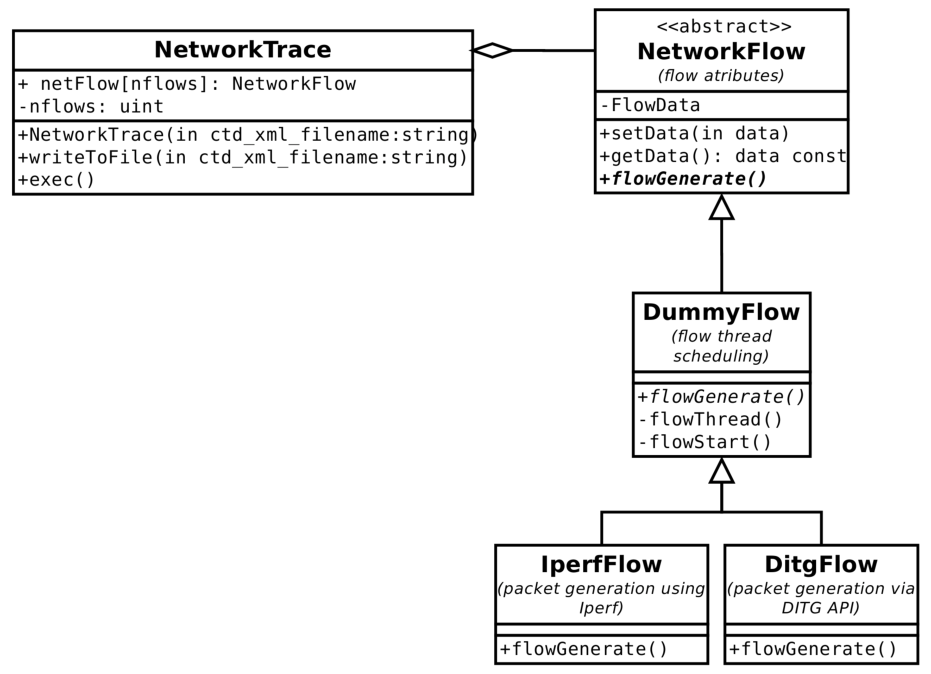
\includegraphics[height=3.0in]{figures/ch3/trace-flow}
    \caption{Class hierarchy of NetworkTrace and NetworkFlow, which enables the abstraction of the traffic generation model of the traffic generation engine.}
    \label{fig:network-trace-flow-class-diagram}
\end{figure*}


\section{Usage and Use Cases}

SIMITAR works in four different states: as a sniffer, packet injector, client or server. 
When it working as a sniffer, is produces as output a Compact Trace Descriptor file. It may operate over a \textit{pcap} file or an Ethernet interface.

When it operates as a client or as packet injector, it is operating as a traffic generator. The difference is that as a client, the used traffic generator is connection-oriented. It needs to establish a connection with the destination host (the server), before start sending packets. It takes as an input a single destination in the command line, or list of many, in a text file passes as a parameter. Also, it uses the machine IP address as packet's source IP.

Operating as a client, it must take as an input a list of IP or MAC destination addresses, since they will not match with the ones in the original trace. As a packet injector can generate packets on the output interface, without establishing a connection. It uses the original IP and MAC destination and source addresses. As a client, the reproduction of the trace is expected to be poor in the flow level metrics exposed in the chapter ~\ref{ch:literature-review}, since it will use new addresses values. 

The operation of packet injector is still under implementation, and we are using Libtins library. Currently, SIMITAR supports client mode with D-ITG, implemented using its C++ API. We intend to provide support for many others traffic generators, such Iperf and Ostinato.

When operating as a server, it just start-up the traffic generator server, and waits for server connections. Down bellow, we present simple examples of commands used to activate each operation mode.

\begin{minted}[frame=single,
               framesep=3mm,
               linenos=true,
               xleftmargin=21pt,
               tabsize=4,
               fontsize=\scriptsize, 
               breaklines=true]{bash}
# Operation as a sniffer over a Ethernet interface named <ether-interface> 
./simitar --sniffer --if <ether-interface> --out <cdt-name>
# Operation as a client using the traffic generator D-ITG, using a list of destination hosts of a text file
./simitar --client ditg --in <cdt-xml-name> --dst-list-ip <ip-list-file> 
# Operation as a packet injector with uses the Libtins library to craft packets
./simitar --pkt-injection libtins --in <cdt-xml-name> 
# Operation as a server. just runs D-ITG in the server mode.
./simitar --server ditg

\end{minted}

As use cases, we can cite:

\begin{itemize}

\item Generate Background traffic with D-ITG: SIMITAR can work to generate background traffic over a network when it receives many addresses as input. If each destination is reachable, D-ITG will establish a connection with each destination, and recreate flows as described in the CDT file. 

\item Stress a Device Under Test (DUT): It can be used to stress a single device with a more self-similar realistic traffic. The CDT file can be manually modified to change some aspects of the traffic, such as the number os packets or throughput applied by the traffic generator of each flow. Some undesirable features such as Stochastic models or lesser flow may be taken out, SIMITAR does not have constraints on a number of flows and Stochastic models adopted (but must have at least one).

\item Generate synthetic \textit{pcap} files: Using virtual interfaces, we can reproduce a traffic, and capture it with a sniffer tool, such as Tcpdump, Wireshark or Tshark. We plan to automatize this process as a future work, with an operation mode of \textit{pcap} generator. To do this we are going to use Mininet to create the virtual interfaces and Libtins to inject packets.

\end{itemize}




